\section*{Descripcion a alto nivel}

\usebeamerfont{serif}


\subsection*{Algoritmo de Búsqueda}

\begin{frame}
    \frametitle{Algoritmo de Búsqueda: }

La búsqueda está basada en el modelo vectorial de recuperación de la información SRI, 
utilizando el TF-IDF (frecuencia de término - frecuencia inversa
 de documento), el cual determina la relevancia de una palabra asociada 
 a un documento en una determinada colección, sumado a la Similitud del Coseno, método mediante el cual se asigna un peso a cada documento y se establece un ranking de resultados según la consulta del usuario.

 \begin{figure}[h]
    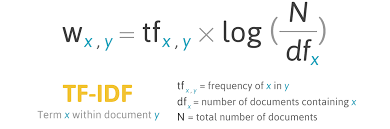
\includegraphics[width=60mm]{sections/descarga.png}
    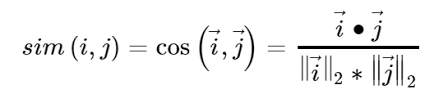
\includegraphics[width=50mm]{sections/descarga (2).png}
 \end{figure}

\end{frame}

 \subsection*{Ventajas del modelo}
 \begin{frame}
    \frametitle{Ventajas del Modelo vectorial}

    \begin{itemize}
         \item Permite una recuperación parcial, es decir, que los documentos se ordenan según su grado de relevancia con la consulta.
\item Es flexible y adaptable, ya que se pueden incorporar diferentes pesos para los términos, según su frecuencia, importancia o discriminación
\item Es eficiente y escalable, ya que se pueden utilizar estructuras de datos e índices que facilitan el cálculo de la similitud
    \end{itemize}


\end{frame}

\section*{MoogleEngine}
    \begin{frame}
        \frametitle{\emph{Estructura de \textbf{MoogleEngine:}}}
    \subsection*{Clases Principales : }
    \framesubtitle{\Large{Clases Principales:}}
        
\begin{block}{\underline{Clase Documento}}
    Esta clase es la encargada de gestionar todo lo relativo a los documentos sobre los que se realizaran las consultas, los carga en memoria y los procesa ,separando los términos que aparecen en los textos , normalizándolos , extrayendo las raíces de estas palabras en una lista para facilitar su posterior uso.

    \begin{beamerboxesrounded}{\color{red}Metodos que incluye:}
        Brinda métodos para obtener una lista de las posiciones donde aparece un término en el documento, su frecuencia, si existe dicho término en el documento y la distancia mínima en el documento entre dos términos. También tiene métodos para obtener la cantidad de veces que aparece la raíz de la palabra y si existe. El método ExtraerOracion extrae del texto del documento una oración con la mayor cantidad de palabras posibles de una lista que le pasamos (consulta) y que se utiliza para buscar el (snipet)fragmento del texto que se devuelve junto con los resultados de la búsqueda.

    \end{beamerboxesrounded}
        
\end{block}
    
    \end{frame}

    \begin{frame}
        \begin{figure}[h]
        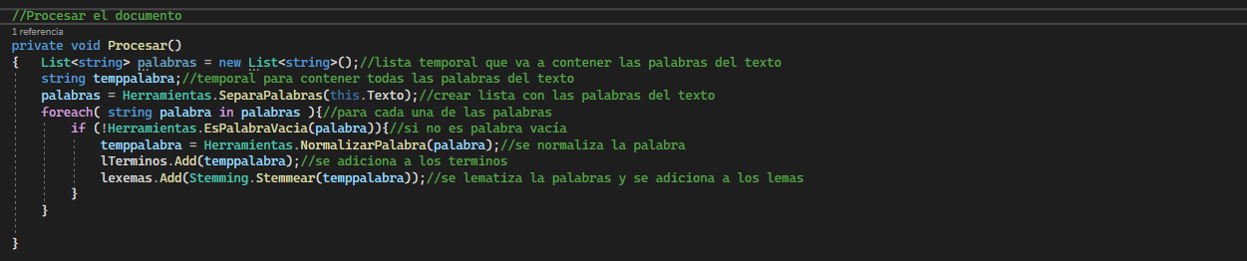
\includegraphics[width=200mm]{Imagen1.png}
        \caption{\textbf{Metodo "Procesar" perteneciente a \underline{Documento}}}     
        \end{figure}
    \end{frame}

    \begin{frame}
        \begin{block}{\underline{Clase QUERY    }}
            Esta clase es la encargada de gestionar todo lo relativo a las consultas. Almacena el texto de la consulta y los términos que aparecen en la misma. 
                  
            \begin{beamerboxesrounded}{\color{red}Al llamar a su constructor se le pasa la consulta ,de la cual:}
\begin{itemize}
    \item Se eliminan las palabras vacías
    \item Se normalizan los términos
    \item Se procesa el uso de operadores (en caso de que existan)
\end{itemize}        
            \end{beamerboxesrounded}
\begin{figure}
    
\includegraphics[width=50mm]{Imagen2.png}
    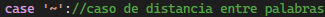
\includegraphics[width=50mm]{Imagen3.png}
    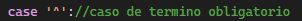
\includegraphics[width=50mm]{Imagen4.png}
    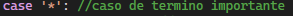
\includegraphics[width=50mm]{Imagen5.png}
    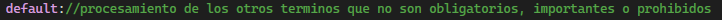
\includegraphics[width=110mm]{Imagen6.png}
\end{figure}               
        \end{block}
    \end{frame}

\begin{frame}
        \frametitle{\huge{Clase \underline{\textbf{Núcleo}}}}
       
      \begin{block}{}
            Esta clase es el núcleo del proyecto , la más importante.

Al llamar a su constructor se crea la lista de documentos, los cuales se procesan y quedan listos para las consultas. Este método es invocado una vez cuando se inicia la aplicación y deja ordenada toda la información para cuando se realicen las consultas.

El método \emph{RealizarConsulta} es el utilizado para realizar una consulta al grupo de documentos de la colección. Se le pasa como parámetro la consulta que se va a realizar y retorna un arreglo de \emph{SearchItem} con los resultados de la \emph{ConsultaRealizada} dependiendo de la información almacenada. 
           \begin{figure}
                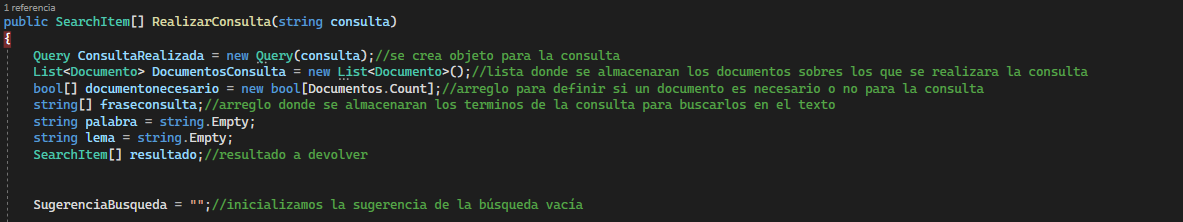
\includegraphics[width=120mm]{Imagen7.png}
            \end{figure}
        \end{block}

\end{frame}

 \begin{frame}
    
    \frametitle{\color{red}Al realizar el usuario una consulta, el proceso realizado por el programa es el siguiente:}
\begin{beamerboxesrounded}{}
        \begin{enumerate}
            \item Del total de documentos de la colección, buscamos los documentos que tengan al menos un término de la consulta. Si no tienen ningún término, el peso del documento será 0, por lo que no nos interesan ya que no aportan ninguna información 
            \item Los documentos obtenidos en el paso anterior son filtrados para eliminar del grupo aquellos que tengan términos prohibidos o no tengan términos obligatorios (según los operadores). 
            \item  Se crea el vector TF de la consulta.             
            \item Se crea la matriz con los vectores TF de los documentos 
            \item Realizamos la revisión de la matriz TF de los documentos antes de pasarla al cálculo de los pesos , debido a que si hay alguna columna en cero significa que el término no se encontró en ningún documento y esto haría una división por 0 que invalidaría el cálculo \textbf{(APARTADO PARA EXPLICAR LA REVISION DE LA MATRIZ)}       
        \end{enumerate}
        \end{beamerboxesrounded}
\end{frame}

\begin{frame}
\frametitle{Luego de este proceso solo queda:}
\begin{block}{}
    \begin{itemize}
    \item Ordenar los documentos de mayor a menor de acuerdo a los pesos de cada uno
    \item Crear el arreglo de SearchItem, incluyendo fragmento del texto que se devuelve junto con los resultados de la búsqueda. 
\item Se devuelven los resultados
\end{itemize}
\textbf{\color{orange}Metodos crucuiales que intervienen:}
\begin{figure}[h]
    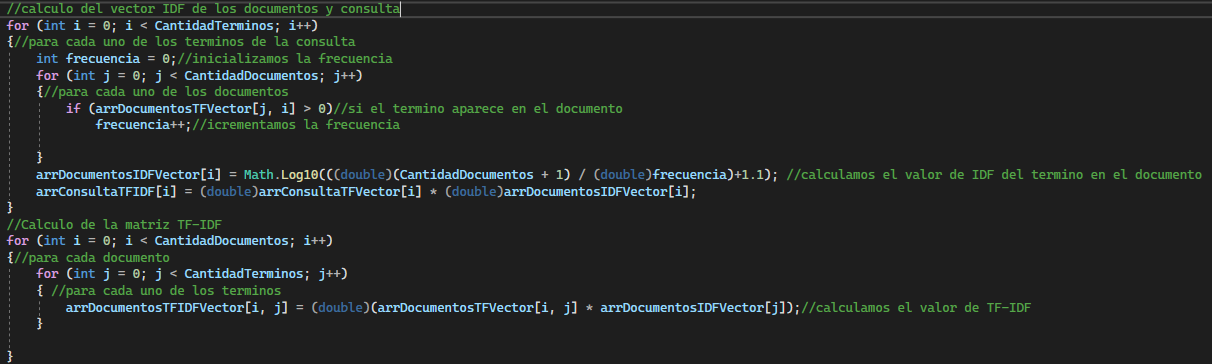
\includegraphics[width=70mm]{Imagen8.png}
    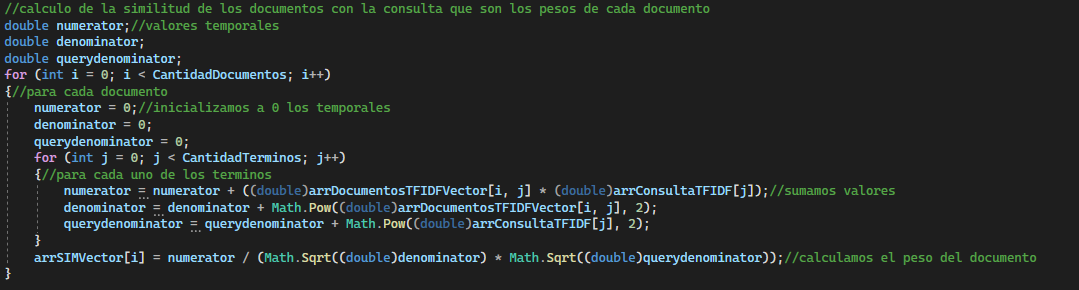
\includegraphics[width=90mm]{Imagen9.png}
\end{figure}
\end{block}

\end{frame}

\subsection*{Clases Auxiliares}

\begin{frame}
    \frametitle{\emph{\huge{Clases Auxiliares}}}
\framesubtitle{Brindan funcionalidades al proyecto,encapsulan procesos necesarios por las CLASES PRINCIPALES y evitan repeticion innecesaria de código.}

\begin{block}{\underline{Clase Herramientas:}}
    Esta clase es la encargada de brindar al resto de las clases propiedades y métodos que son utilizados de forma indistinta. En ella se definen los caminos de los archivos de los documentos, métodos básicos del procesamiento de los textos y de cálculos, tipos de datos nuevos, Distancia de Damerau-Levenshtein etc.
\end{block}
\begin{block}{\underline{Clase Stopwords:}}
    Creamos una lista de las palabras que aparecen en los documentos y de las veces que aparece cada una. Tomando en cuenta las veces que aparece cada palabra, ordenamos este listado de menor a mayor y buscamos la mayor cantidad posible de palabras que aparezcan en los documentos y que la suma de sus apariciones sea menor que la suma de las apariciones de las palabras que más aparecen. Esto nos brinda un punto de corte para diferenciar las palabras vacías de las palabras buenas.
\end{block}
\end{frame}

\begin{frame}
    \begin{block}{\underline{Clase Stemming:}}
        Es la encargada de etraer la raíz o lexema de cada palabra 
    
    \end{block}
\end{frame}

\section*{Funcionalidades adicionales:}

\begin{frame}
    \frametitle{Funcionalidades adicionales:}
    \begin{block}{\color{red}El proyecto cuenta con varios operadores para mejorar la búsqueda del usuario:}
    \begin{figure}
        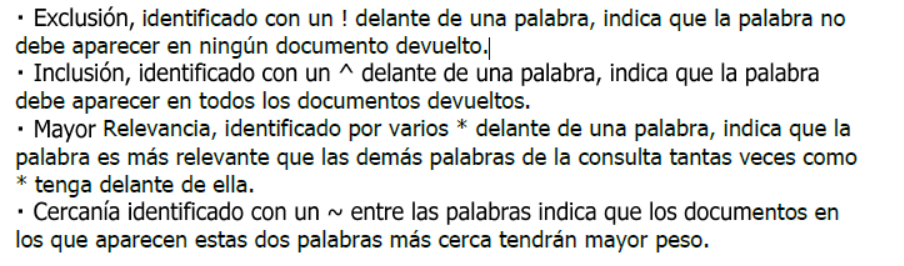
\includegraphics[width=100mm]{Imagen10.png}
    \end{figure}
    \end{block}
    
    \begin{block}{\color{orange}{Sugerencia para corregir la búsqueda del usuario:}}
    En caso de que la búsqueda no coincida con ningún valor almacenado , tenemos este “corrector ” para garantizar de que aún habiendo palabras erróneas  en la consulta el programa intuya el termino correcto que el usuario quiso expresar en la consulta. 
 \color{red}Esta también se apoya en el Stemming para realizar una segunda búsqueda de sugerencia , ya que pueden existir terminos muy largos que su palabra primitiva aparezca en la coleccion pero no pueda ser devuelta por el metodo Damerau-Levenshtein
\end{block}

\end{frame}

